% !TeX spellcheck = en_US
\documentclass[a4paper,twocolumn]{article}

\usepackage{fullpage}
\usepackage{fourier}
\usepackage{amsmath}
\usepackage{xcolor}
\usepackage{graphicx}
\usepackage{titlesec}
\usepackage{hyperref}
\usepackage{cleveref}

\titleformat{\subsection}[hang]{\large\bfseries}{\alph{subsection})\quad}{0pt}{}

\newcommand{\twodo}[1]{\textcolor{red}{\textbf{todo:} #1}}
\newcommand{\subtask}[2]{\paragraph{#1)} \textit{#2} \newline}

\title{\textbf{Exercises for Image Processing 1}\\Problem Sheet 3}
\author{Axel Brand\\6145101 \and Nourhan Elfaramawy\\6517858 \and Sibel Toprak\\6712316}

\begin{document}
	\maketitle
	
	\section{Perspective Transforms}
	
	% % % % %
	\subtask{a}{Show that 3D straight lines in a scene are depicted as 2D straight lines in an image by perspective projection.}
	
	A straight line in a three-dimensional scene can be specified in terms of an offset vector $\vec{o}$  with respect to the origin of the reference coordinate system and a direction vector $\vec{d}$ like so:
	\begin{align*}
		\vec{p} = \vec{o} + s \cdot \vec{d}
	\end{align*}
	
	Here, $s$ denotes a scalar factor with the help of which any point $\vec{p}$ along that straight line can be computed. The equation can also be written component-wise:
	\begin{align*}
		p_x &= o_x + s \cdot d_x \\
		p_y &= o_y + s \cdot d_y \\
		p_z &= o_z + s \cdot d_z
	\end{align*}
	
	Applying perspective projection equations to these components and expanding them results in the following:
	\begin{align*}
		p_{x}^{\prime} &= \frac{f}{p_{z}} \cdot p_{x} 
		&= (\frac{f}{p_{z}} \cdot o_x) + s \cdot (\frac{f}{p_{z}} \cdot d_x) \\
		p_{y}^{\prime} &= \frac{f}{p_{z}} \cdot p_{y}
		&= (\frac{f}{p_{z}} \cdot o_y) + s \cdot (\frac{f}{p_{z}} \cdot d_y) \\
		p_{z}^{\prime} &= f
	\end{align*}
	
	$f$ is the so-called focal length, which is the distance between the image plane and the optical center with respect to the camera coordinate system. $p_{z}^{\prime}$ is redundant, because it has the same value, $f$, for all image points. Thus, the $p_{z}^{\prime}$ component can be ignored. What matters are the $p_{x}^{\prime}$ and $p_{y}^{\prime}$ components. Their projection equations can be rewritten as follows:
	\begin{align*}
		\begin{pmatrix}
		p_{x}^{\prime} \\
		p_{y}^{\prime}
		\end{pmatrix}
		=
		\begin{pmatrix}
		\frac{f}{p_{z}} \cdot o_x \\
		\frac{f}{p_{z}} \cdot o_y
		\end{pmatrix}
		+ s \cdot
		\begin{pmatrix}
		\frac{f}{p_{z}} \cdot d_x \\
		\frac{f}{p_{z}} \cdot d_y
		\end{pmatrix}
	\end{align*}
	
	The resulting equation indeed describes a straight line in the two-dimensional image plane. \hfill $\square$
	
	% % % % %
	\subtask{b}{Show that the perspective projections of parallel 3D straight lines in a scene intersect in a single point, the vanishing point. In which case is the vanishing point located in infinity?}
	
	
	\begin{figure*}
		\centering
		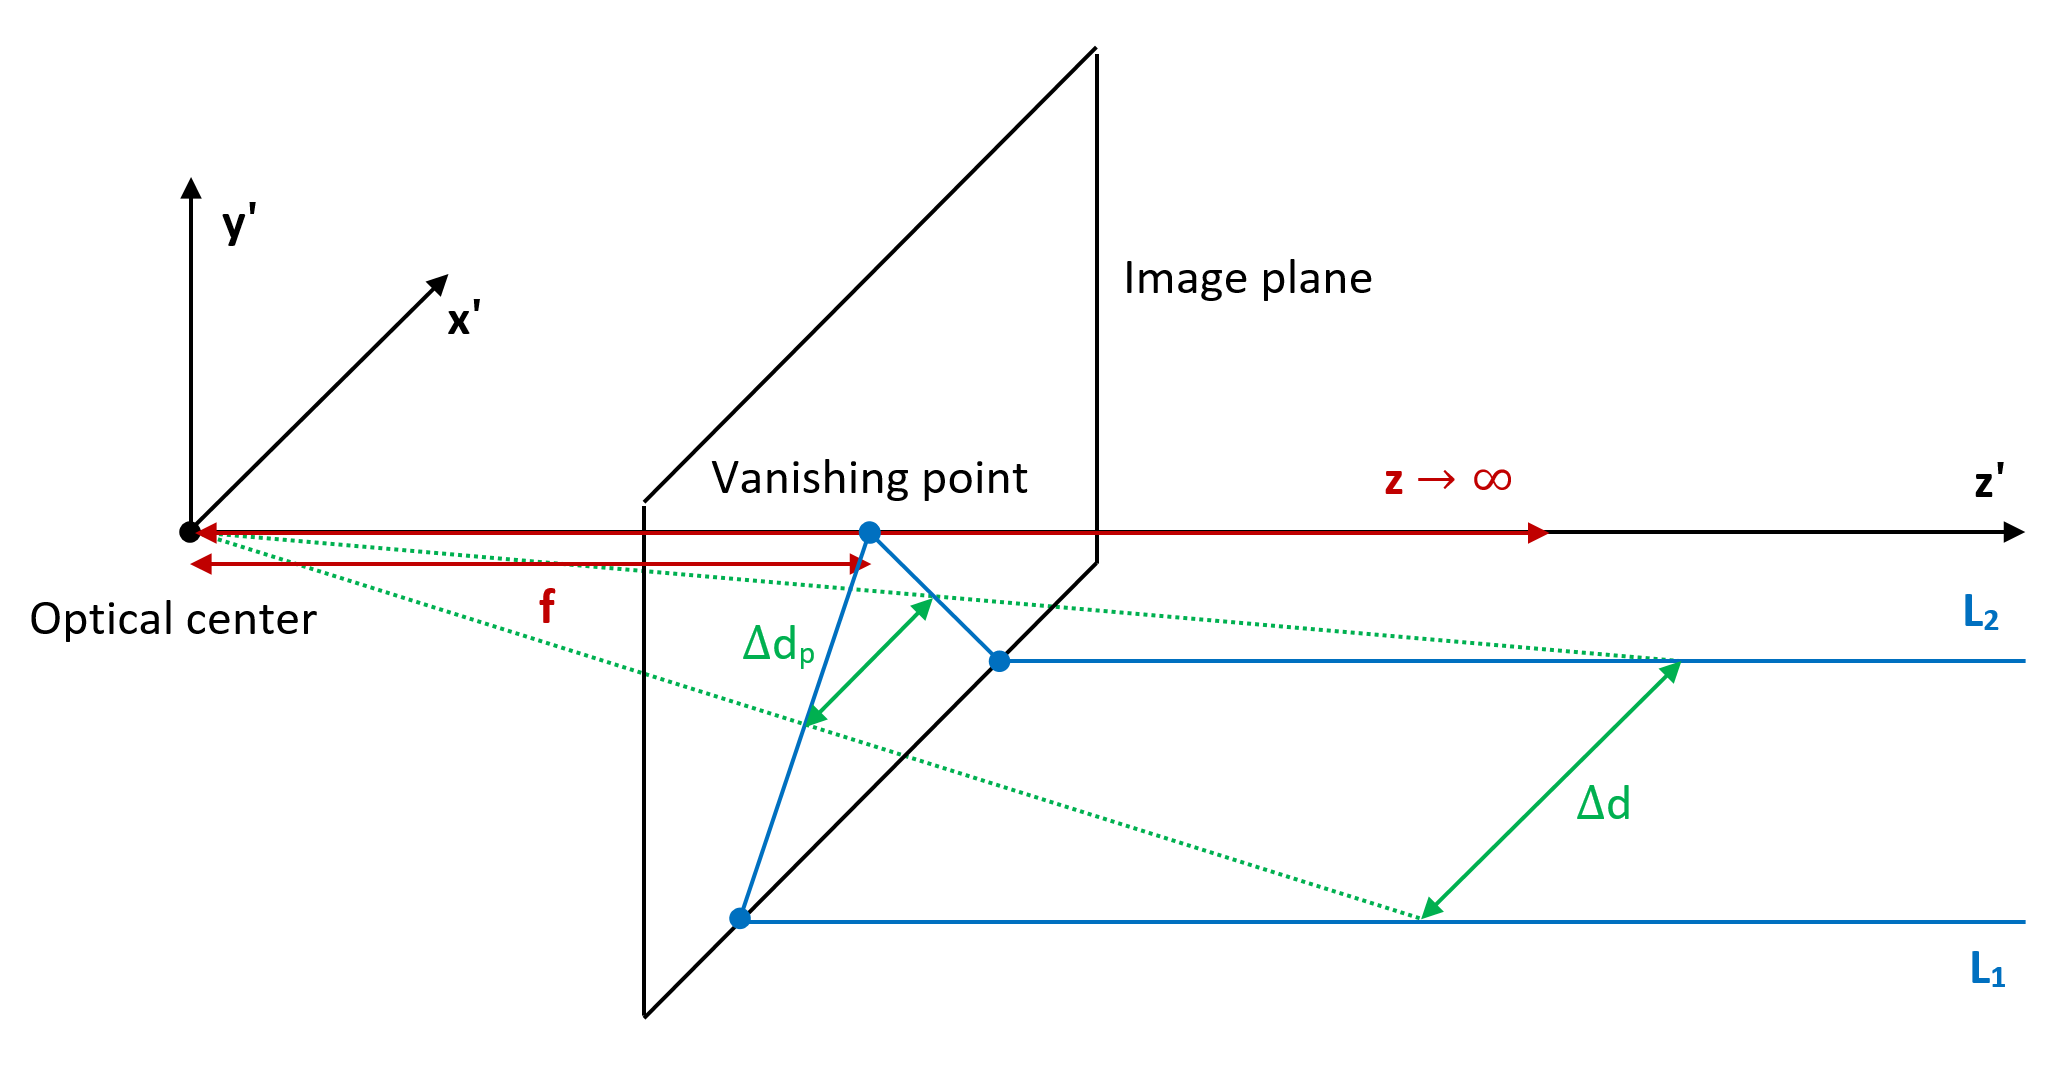
\includegraphics[width=\textwidth]{vanishing_point.png}
		\caption{Perspective projections of parallel 3D straight lines in a scene onto an image plane. $f$ denotes the focal length.}
		\label{fig:vanishing_point}
	\end{figure*}
	
	\textcolor{gray}{\textbf{Remark:} It turned out that each of us interpreted this task differently. Because we were not sure which of our interpretations is the correct one, we decided to provide all of them here.}
	
	\paragraph{Interpretation 1:} The general setting is shown in \Cref{fig:vanishing_point}: We have two straight blue lines in the scene that are parallel to each other called $L_1$ and $L_2$. We select one point along each of the two lines such that connecting the two of them yields a straight line segment, the green one, that is parallel to the image plane. We will refer to the point on $L_1$ as $p_1$ and the point on $L_2$ as $p_2$.
	
	Furthermore, let $\Delta d$ be the length of this connecting line segment. Because of the parallelism between the two straight lines, $\Delta d$ is always constant even if the green line between $p_1$ and $p_2$ moves towards infinity along $z^{\prime}$.
	
	The image points corresponding to the scene points $p_1$ and $p_2$ respectively are determined as follows: Each point is connected to the optical center by a straight line segment (the green dotted lines n \Cref{fig:vanishing_point}). The points at which these straight line segments intersect with the image plane are the image points. Let $\Delta d_p$ be the distance between the image points of $p_1$ and $p_2$.
	
	Using the intercept theorem, we can infer the following equation:
	\begin{align*}
		\frac{\Delta d_p}{\Delta d} = \frac{f}{z} &\Leftrightarrow
		\Delta d_p = \frac{f}{z} \cdot \Delta d \\
		z \rightarrow \infty &\Rightarrow \Delta d_p \rightarrow 0
	\end{align*}
	
	Basically, the more the straight line segment of constant length $\Delta d$ moves away from the image plane along the $z$ axis, the more the length $\Delta d_p$ of its projection converges to zero. That is, the image points corresponding to the scene points $p_1$ and $p_2$ converge to what is called the vanishing point.


	%In the case of \textbf{Orthographic projection}. Then all lines which are parallel in the real world are also parallel in the projected world.
	
	\paragraph{Interpretation 2:} Parallel lines in space project perspectively onto lines that on extension intersect at a single point in the image plane called vanishing point or point at infinity. The vanishing point of a line depends on the orientation of the line and not on the position of the line. The vanishing point of any given line in space is located at the point in the image where a parallel line through the center of projection intersects the image plane.
	
	By inserting into a Cartesian scene a set of parallel lines that are not parallel to any of the three axes of the scene, a new distinct vanishing point is created. Therefore, it is possible to have an infinite-point perspective if the scene being viewed is not a Cartesian scene but instead consists of infinite pairs of parallel lines, where each pair is not parallel to any other pair.
	
	% % % % %
	\subtask{c}{What shapes have the perspective projections of spheres? Justify your answer.}
	
	Given a sphere in the scene, we can visualize the set of points which connect the optical center of the camera to the edges of the visible hemisphere of the sphere as being a geometrical cone with the same radius and the top angle lying on the center. This cone is sliced by the image plane and rendered 2- dimensional exactly how the sphere is represented on the resulting picture.
	
	So given a not null focal distance, a normal optical axis to the image plane and a sphere lying on a side of the image plane, the sphere will result in a circle in the image if its center point lies on the optical axis of the camera, thus the geometrical cone is then sliced by a plane parallel to its base, while in any other case the sphere will be an ellipse.


	
	Spheres are looking like ellipses in a 3D projection:
	
	\begin{figure}[h!]
		\centering
		%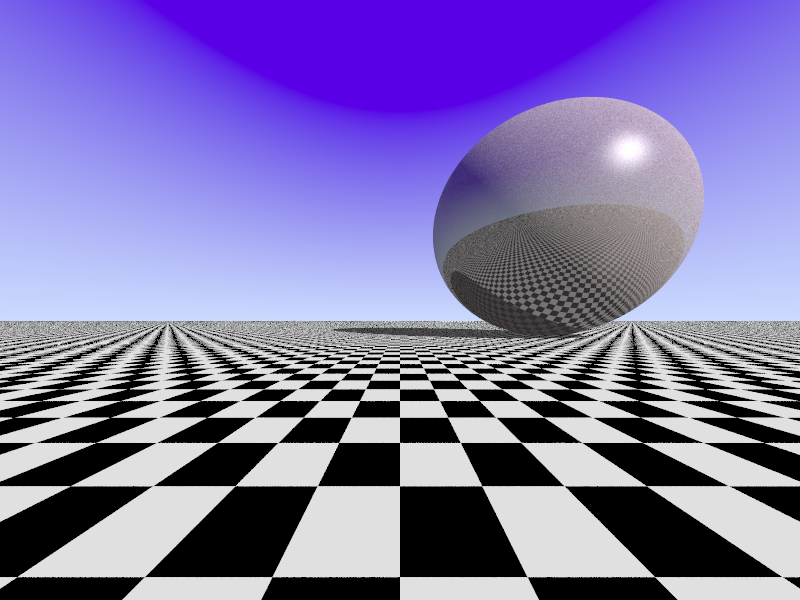
\includegraphics[width=0.7\textwidth]{E03.png}
		\caption{Sphere rendered with perspective projection in POV-Ray.}
	\end{figure}
	
	
\end{document}
